\chapter{Metodología}
En el presente capítulo se explicará la teoría y práctica detrás de los métodos que se ocuparon en esta tesis para realizar el análisis de los medios porosos heterogéneos. En primera instancia se estudia el conjunto de bibliotecas FeniCS usadas para implementar el método de elemento finito, las funcionalidades de cada módulo y el uso de otras herramientas para definir la heterogeneidad del sistema. Posteriormente, se aborda el método de elemento finito para resolver la ecuación de flujo, su teoría y su aplicación a partir de la formulación tradicional.




\section{Bibliotecas FEniCS}

El conjunto de bibliotecas FEniCS es el resultado de un esfuerzo en conjunto de varios investigadores y programadores que buscan aumentar la eficiencia en la resolución mediante el método de elemento finito de ecuaciones diferenciales parciales (EDP) que modelan fenómenos físicos a partir de la implementación de funciones en los lenguajes de programación \textit{python} y \textit{C++} \cite{Logg2012}.
\\
\\
El proyecto FEniCS surge en el año 2003 como una colaboración de la Universidad Tecnológica de Chalmers y la Universidad de Chicago; sin embargo , su utilidad y eficacia produjo que varias universidades e institutos alrededor del mundo colaboraran para aportar más herramientas y funcionalidades al proyecto. Inicialmente, FEniCS consistía de dos bibliotecas, DOLFIN y FIAT, que realizaban el trabajo de automatizar la resolución de las EDP. Debido al crecimiento del proyecto las bibliotecas centrales que ocupa la plataforma FEniCS son DOLFIN, FFC, FIAT,Instant,UFC y UFL. Otros componentes de FeniCS ocupados en el proyecto son SyFi/SFC, FErari,ASCoT,Unicorn,CBC.block,CBC.RANS, CBC.Solve y DOLFWAVE. Los componentes principales de FeniCS serán descritos a continuación:
\\
\\
\textbf{DOLFIN} es la interfaz principal de usuario de FeniCS. La implementación de las otras bibliotecas de FeniCS se realiza atraves de DOLFIN, esta nos provee un ambiente para resolver las ecuaciones diferenciales parciales e implementa partes del núcleo principal de FEniCS, como las estructuras de datos y algoritmos para las mallas y el ensamblado de los elementos finitos. El interfaz de usuario de DOLFIN resulta simple y consistente de usar, además funciona para usar junto a otros componentes externos y realizar la comunicación entre ellos.


\begin{figure}[ht!]
\centering
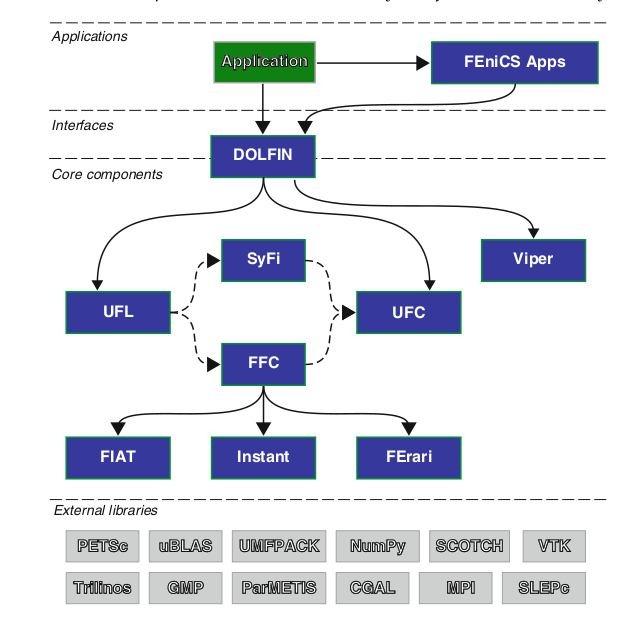
\includegraphics[scale=0.55]{Figura14.png}
\caption{ Esquema de la estructura de FEniCS (Logg et al, 2012) }
\label{Figura14:2}
\end{figure}

En la figura \ref{Figura14:2} podemos observar cómo interactúa DOLFIN con las demás componentes de FEniCS; DOLFIN se comporta como la interfaz donde se realiza la comunicación a partir de un lenguaje de programación que puede ser tanto Python como C++. Además, también funciona como núcleo de FEniCS ya que permite la comunicación con otros componentes fundamentales . Por ejemplo, la formulación variacional de nuestra ecuación diferencial parcial se expresa a partir de DOLFIN, donde se comunica con la biblioteca UFL que la códifica y realiza la compilación con las bibliotecas FFC o SFC, donde se genera un código UFC que DOLFIN ocupa para ensamblar los sistemas de ecuaciones lineales para cada elemento finito. Por lo anteriormente descrito, DOLFIN también necesita de bibliotecas externas ajenas al proyecto FEniCS como las que nos ayudan a resolver problemas de algebra lineal como PETSc y Trilinos, además de bibliotecas generadoras de mallas como ParMETIS y SCOTCH.

\begin{figure}[ht!]
\centering
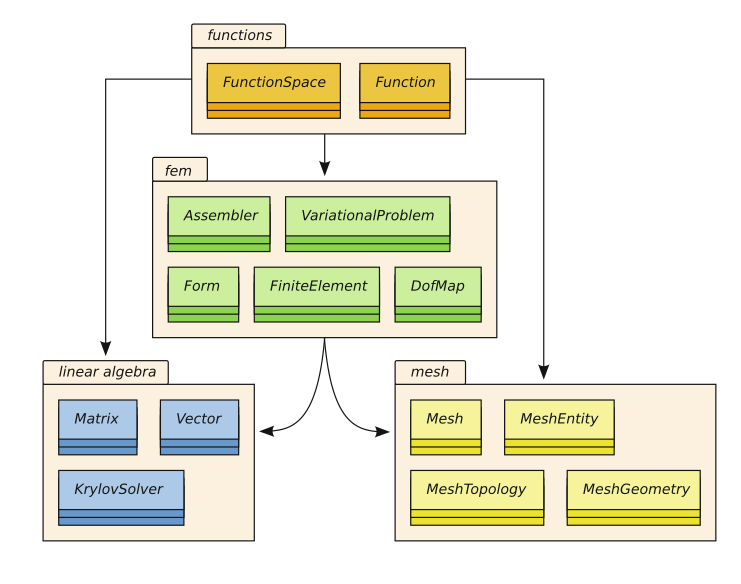
\includegraphics[scale=0.60]{Figura15.png}
\caption{ Funciones y clases de DOLFIN (Logg et al, 2012). }
\label{Figura15:2}
\end{figure}

FEniCS maneja dos tipos de interfaces a partir del lenguaje de programación que se prefiera ocupar: Python y C++ . En esta tesis se usara la interfaz implementada como modulo de Python  debido a que se trata de un lenguaje práctico, interpretado y que permite una programación orientada a objetos al que se puede sacar mayor provecho que un paradigma estructurado. En la figura \ref{Figura15:2} podemos observar las principales funciones y clases en FEniCS que podemos ocupar para resolver nuestras ecuaciones diferenciales, desde funciones que nos ayudan a generar un espacio de funciones hasta la creación de mallas que representan nuestro dominio de estudio.
\\

Otros componentes de FEniCS son \textbf{UFL} (Unified Form Language) que implementa a partir de un lenguaje abstracto, las formulaciones variacionales de ecuaciones diferenciales para cada elemento finito y el espacio de elementos finitos hacia una notación cercana a la matemática y \textbf{UFC}(Unified Assembly-Code) que evalua y ensambla formas variacionales de elementos finitos, escrita en C++ esta componente define la estructura y firma de código generados por algún compilador del sistema (FFC y SFC) para DOLFIN, la versatilidad de UFC debido a su estructura en C++ permite que pueda usarse con múltiples bibliotecas y en una amplia gama de problemas de elementos finitos. En la figura \ref{Figura14:2} podemos observar como DOLFIN interactua con UFL donde se realiza la implementación del problema, se codifica para posteriormente ser compilado y ensamblado por UFC, también es posible hacer el ensamblado de forma directa en UFC sin necesidad de pasar por UFL si la implementación se realiza a partir de una biblioteca externa.
\\

Entre el proceso de codificación y ensamblaje, tenemos el proceso de compilación que en FEniCS se aplica a partir de \textbf{FFC}(FEniCS Form Compiler) o \textbf{SyFi}(Symbolic Finite Elements) en conjunto con su compilador \textbf{SFC}(SyFi Form Compiler). La componente FFC es el motor principal de FEniCS que genera un código C++ eficiente a partir del lenguaje abstracto proporcionado por UFL y genera la salida UFC. Este compilador se apoya principalmente de otros componentes como \textbf{FIAT}(Finite Element Automatic Tabulador) que a partir de la biblioteca externa NumPy, construye númericamente las funciones base de elementos finitos, la componente \textbf{Instant} que es un pequeño modulo en Python para la compilación de código "Just-in-time" y la componente \textbf{FErari}(Finite Element ReARrangemnts of Integrals) que permite la opción de aplicar optimizaciones basados en el estudio de graficos en tiempo de compilación para reducir el tiempo de ejecución sin afectar en el resultado final.
\\
\\
Las componentes SyFi y SFC son ocupadas para definir simbolicamente elementos finitos para ser compilado después, funcionan de forma análoga a las bibliotecas FFC y FIAT donde a partir de un código UFL se obtiene la salida para UFC y ser ensamblado por DOLFIN. La implementación de SyFi y SFC resulta ser más útil para lenguaje C++, mientras que para Python que es el lenguaje con el que se trabajara, resulta más eficiente usar el compilador FFC \cite{Perez2018}


\section{Método de elemento finito}

Las ecuación de flujo es una ecuación diferencial parcial que es posible resolver de forma analítica (tomando ciertas restricciones) o utilizando métodos númericos, donde tipicamente se implementa el método de diferencias finitas que resulta el más fácil e intuitivo de utilizar. El principal problema de emplear diferencias finitas es la poca disposición que tiene el método para resolver la ecuación en un dominio con geometría compleja; esto es importante ya que generalmente queremos obtener resultados en cuencas o estructuras geológicas que no es posible modelar con formas rectangulares. El método que se empleará en esta tesis es el método de elemento finito cuyo empleo resulta muy atractiva debido a su enfoque en sus elementos individuales, que pueden tener geometrías muy complejas, además de proporcionar diferentes variaciones del método para cada situación en particular.
\\

El método de elementos finitos, remonta hacia 1915 con los estudios sobre EDP's del matemático ruso Boris Galerkin, donde anteriormente un estudio similar habia sido desarrollado por el ingeniero también ruso Buvnov. El método de Bubnov-Galerkin consistia en convertir un problema analitico como lo es una ecuación diferencial en un problema discreto a partir de polinomios globales y los principios variaciones dados por Leibniz, Euler, Lagrange, Ritz y Rayleigh. El método de Galerkin evolucionó hasta el uso de espacios polinomiales, que es el método al que actualmente se le conoce como Elementos Finitos. El método fue ocupado principalmente en los años 50's para el análisis estructural principalmente por el matemático alemán Richard Courant. Posteriormente, debido a la flexibilidad del método, matemáticos e ingenieros comenzaron a desarrollar diferentes variaciones del método y a desarrollar un amplio marco teórico sobre el mismo, creando un  refinado marco de refencia para la resolución de ecuaciones diferenciales a partir de su análisis númerico. En la actualidad aún se sigue profundizando en el desarrollo del método, donde se busca la eficiencia en la discretización de problemas variacionales mixtos para el cálculo simultaneo del flujo \cite{Logg2012}.

\subsection{Formulación integral}

Al igual que el método de diferencias finitas, el objetivo es obtener la solución del problema en cada punto de la malla definida, lo cuál logramos al obtener un sistema de ecuaciones algebraicas cuyo número de soluciones sea igual al número de incognitas dentro de nuestro dominio de estudio. Para lograr esto, el primer paso de cualquier método de elementos finitos es reeplantear la ecuación diferencial para obtener una formulación integral a partir de diferentes métodos, los más conocidos son el método de residuos ponderados y el método variacional \cite{Istok1989}. 
\\

Para abordar el método de residuos ponderados y variacional, plantearemos una ecuación diferencial general como un operador $L$ aplicado a una función $u$ que es la solución del problema de la siguiente forma:

\begin{equation}
\label{eqn:fe1}
 \ L^{p}(u(x,y,z))=F(x,y,z)
\end{equation}

Donde el operador $L$ representa un polinomio diferencial y p el orden de la EDP ($L=(D^{p}+D^{p-1}+D^{p-2}...+D+C$) y la solución $u$ es una función de las coordenadas $(x,y,z)$ y la función $F(x,y,z)$ es el término no homogéneo de la ecuación. El método de residuos ponderados consiste en plantear una solución aproximada $\hat{u}$ cuya sustitución en la ecuación genere un residuo $R(x,y,z)$ de la siguiente forma: 

\begin{equation}
\label{eqn:fe2}
 \ L^{p}(\hat{u}(x,y,z))-F(x,y,z)=R(x,y,z)
\end{equation}

Para minimizar el residuo mostrado en la ecuación \ref{eqn:fe2}, obtendremos una función $v(x,y,z)$ cuya caracteristica principal sea que la integral de su producto con el residuo sobre todo el dominio sea igual a cero, como lo muestra la ecuación \ref{eqn:fe3}. 

\begin{equation}
\label{eqn:fe3}
  \displaystyle\int_{\Omega}^{} R(x,y,z)v(x,y,z)\, d\Omega = 0
\end{equation}

La función $v(x,y,z)$ es también llamada función de peso, y tiene que cumplir ciertas características, que seran explicadas más adelante, para poder minimizar el residual. Recordando que el residual es igual a la ecuación diferencial donde la solución general es sustituida por la aproximada, entonces, sustituyendo la ecuación \ref{eqn:fe2} en \ref{eqn:fe3}, obtenemos el siguiente resultado:

\begin{equation}
\label{eqn:fe4}
  \displaystyle\int_{\Omega}^{} [L^{p}(\hat{u}(x,y,z))-F(x,y,z)] v(x,y,z)\, d\Omega = 0      
\end{equation}

Uno de los puntos escenciales para obtener la formulación integral de la ecuación diferencial, es la definición de la función solución aproximada $\hat{u}(x,y,z)$, este punto es crucial para el método y es el que le da sentido a su nombre, ya que la solución aproximada en cada punto del dominio es una combinación lineal de su valor en otros puntos (definida por una malla) y funciones de interpolación, como se muestra en la ecuación \ref{eqn:fe5}.

\begin{equation}
\label{eqn:fe5}
    \hat{u}=\displaystyle\sum_{i=1}^m  N_{i}(x,y,z){\hat{u}_{i}}        
\end{equation}

Donde $m$ es el número de nodos, $N(x,y,z)$ es la función de interpolación para cada punto y $\hat{u}_{i}$ es el valor desconocido de la función solución en cualquier punto del dominio. La resolución de la ecuación pasa de ser un problema analítico a un problema numérico cuando hacemos la discretización del dominio a partir de una malla, donde a diferencia de otros métodos numéricos para EDP, la discretización se realiza a partir de elementos que pueden adquirir diferentes formas y tamaños, por lo que la ecuación \ref{eqn:fe5} que determina la solución del problema, la adaptamos para obtener la solución por cada elemento donde el dominio fue discretizado. 

\begin{equation}
\label{eqn:fe6}
    \hat{u}^{e}=\displaystyle\sum_{i=1}^n  N_{i}^{e}(x,y,z){\hat{u}_{i}}        
\end{equation}

A partir de la ecuación \ref{eqn:fe6} podemos obtener la solución en cada punto dentro del dominio donde el problema se ve definido a partir de la formulación integral planteada en la ecuación \ref{eqn:fe4}. 
\\
\\
Habiendo definido entonces la solución aproximada $\hat{u}$, y siendo conocido el operador diferencial $D$ y la función independiente $F(x,y,z)$, queda definir la función de peso; la más ocupada en términos generales es el descrito por el método de Galerkin que como se comentó al principio del tema, ocupa un espacio de funciones polinomiales para hacer la aproximación a la solución y ocupa las mismas funciones para definir las funciones de peso, de esta forma, las funciones de peso serán iguales a la funciónes de interpolación de cada punto. Obteniendo la siguiente formulación integral:

\begin{equation}
\label{eqn:fe7}
  \displaystyle\int_{\Omega}^{} [D^{p}(\hat{u}(x,y,z))-F(x,y,z)] N(x,y,z)\, d\Omega = 0      
\end{equation}
  
El método de residuales ponderados es el método más intuitivo para explicar cómo se deduce la formulación integral, sin embargo, el método variacional abarca el problema desde un enfoque más general, siendo el resultado de trabajos de matemáticos como Ritz y Rayleigh, cuyo enfoque para minimizar la energia debido al trabajo en un sistema físico los llevo a replantear sus EDP a una expresión donde esas condiciones estaban dadas. Para definir el problema variacional de una EDP, es necesario primero definir todo el espacio de funciones donde podriamos encontrar nuestra solución $u(x,y,z)$; sea entonces $L^{2}(\Omega)$ el espacio de funciones definido en nuestro dominio $\Omega$ y  $v(x,y,z){\in}L^{2}(\Omega)$ (usaremos la misma notación que la función de peso), donde además sea posible definir la siguiente operación:

\begin{equation}
\label{eqn:fe8}
 	 \displaystyle\int_{\Omega}^{} (v(x,y,z))^{2}\, d\Omega
\end{equation}

El conjunto de funciones $L^{2}(\Omega)$ es también conocido como espacio de Hilbert \cite{Esparza}, y es en este conjunto de funciones donde se encuentra nuestra solución $u(x,y,z)$.

\begin{equation}
\label{eqn:fe9}
  L^{2}(\Omega)=  \left[ v(x,y,z) : \displaystyle\int_{\Omega}^{} (v(x,y,z))^{2}\, d\Omega < \infty \right] 
\end{equation}

Los espacios de funciones de Hilbert tienen elementos infinitos, por lo que es necesario definir otra operación donde sea posible acotar las funciones y ayudarnos a plantear la formulación integral de la EDP. El nuevo espacio de funciones $H^{1}(\Omega)$ se define de la misma forma que el espacio $L^{2}(\Omega)$, solo agregando que las derivadas de $v(x,y,z)$ pertenezcan al espacio $L^{2}(\Omega)$, dicho de otra forma, se define la operación dada en la ecuación \ref{eqn:fe8} para las derivadas de la función $v(x,y,z)$, este nuevo espacio de funciones, también llamados espacios de Sovolev \cite{Whiteley2017}, se definen de la siguiente forma:

\begin{equation}
\label{eqn:fe10}
   H^{1}(\Omega)=  \left[ v(x,y,z):\displaystyle\int_{\Omega}^{} (v(x,y,z))^{2}\, d\Omega\infty < \infty : \displaystyle\int_{\Omega}^{} (\nabla{\cdot}v(x,y,z))^{2}\, d\Omega < \infty\right]  
\end{equation}

\begin{equation}
\label{eqn:fe11}
   H^{1}(\Omega)=  \left[ v(x,y,z)\in H^{2}(\Omega): \nabla{\cdot}v(x,y,z){\in} H^{2}(\Omega) \right]  
\end{equation}

Con estos espacios definidos, nosotros podemos comenzar a plantear la formulación integral de nuestra EDP. Regresando a nuestra ecuación diferencial, expresada en la ecuación \ref{eqn:fe1}, podemos observar que la solución analítica puede ser expresada como una función que se encuentra en el espacio de Sobolev $H^{1}(\Omega)$, a la solución que cumple estas características es llamada solución debil, y podemos obtener la formulación integral a partir del método variacional multiplicando una función test $v(x,y,z){\in}H^{1}$ en ambas partes de la EDP, obteniendo la siguiente ecuación:

\begin{equation}
\label{eqn:fe12}
  \ L^{p}(u(x,y,z))v(x,y,z)=F(x,y,z)v(x,y,z)
\end{equation}

A partir de la ecuación \ref{eqn:fe12} y debido a las características de las funciones definidas en $H^{1}$, integramos sobre el dominio en ambas partes de la ecuación, obteniendo la formulación integral (ecuación \ref{eqn:fe13}), donde si despejamos el lado derecho y factorizamos la función $v(x,y,z)$, obtenemos la ecuación \ref{eqn:fe14}.

\begin{equation}
\label{eqn:fe13}
  \displaystyle\int_{\Omega}^{} L^{p}(u(x,y,z))v(x,y,z)\, d\Omega = \displaystyle\int_{\Omega}^{} F(x,y,z)v(x,y,z)d\Omega  
\end{equation}

\begin{equation}
\label{eqn:fe14}
 \displaystyle\int_{\Omega}^{} L^{p}(u(x,y,z))v(x,y,z)\, d\Omega - \displaystyle\int_{\Omega}^{} F(x,y,z)v(x,y,z)d\Omega = 0  
\end{equation}

\begin{equation}
\label{eqn:fe15}
 \displaystyle\int_{\Omega}^{} [L^{p}(u(x,y,z))-F(x,y,z)]v(x,y,z)\, d\Omega = 0   
\end{equation}

Donde se puede observar, la ecuación \ref{eqn:fe15} es la formulación integral que se obtuvo con el método de residuos ponderados (\ref{eqn:fe4}). De la misma forma se define la solución aproximada $\hat{u}$ como una combinación lineal, donde las funciones de interpolación $N(x,y,z)$ se consideran una base del espacio de funciones $H^{1}(\Omega)$,  por lo que tienen que cumplir con las condiciones especificadas en la expresión \ref{eqn:fe11}.
\\
\\
Para obtener la formulacion integral final, es necesario tomar en consideración que la función de interpolación $N(x,y,z)$ debe de ser continua y derivable, por lo que para relajar las condiciones de derivabilidad se ocupa la integración por partes en la ecuación \ref{eqn:fe12} . En el caso de un operador derivada de segundo orden $L^{2}$ y asumiendo que el polinomio diferencial solo expresa el componente de mayor orden ($L=D^{2}={\nabla}^{2}$), integramos esta expresión y derivamos la función test $v(x,y,z)$, obteniendo las siguientes expresiones:

\begin{equation}
\label{eqn:fe16}
 \displaystyle\int_{\Omega}^{} {\nabla}^{2}(u(x,y,z))v(x,y,z)\, d\Omega = \displaystyle\int_{\Omega}^{} F(x,y,z)v(x,y,z)d\Omega  
\end{equation}

\begin{equation}
\label{eqn:fe17}
 \displaystyle\int_{\Omega}^{}{\nabla}^{2}(u(x,y,z))v(x,y,z)\, d\Omega = \left. \nabla{u(x,y,z)}v(x,y,z)\right]_{\partial{\Omega}}-\displaystyle\int_{\Omega}^{} {\nabla}u(x,y,z){\nabla}v(x,y,z)d\Omega 
\end{equation}

Como se observa en la ecuación \ref{eqn:fe16}, las condiciones de derivabilidad se relajan y el término extra consiste en la imposición de las condiciones de frontera. Finalmente, se sustituye en la ecuación \ref{eqn:fe15} y obtenemos la formulación variacional para un operador diferencial $L^{2}$.

\begin{equation}
\label{eqn:fe18a}
  \displaystyle\int_{\Omega}^{} {\nabla}u(x,y,z){\nabla}v(x,y,z)d\Omega   = \displaystyle\int_{\Omega}^{} F(x,y,z)v(x,y,z)d\Omega  - \left. \nabla{u(x,y,z)}v(x,y,z)\right]_{\partial{\Omega}} 
\end{equation}

Una generalización aún más amplia se puede obtener al definir la aplicación de las funciones test $v(x,y,z)$ como una forma bilineal $a:H^{1}xH^{1}{\to}\mathbb{R}$  mientras que la parte derecha de la ecuación \ref{eqn:fe18} es una forma lineal y continua $f:H^{1}{\to}\mathbb{R}$. Se dice entonces que $u$ es una solución débil del problema variacional si cumple la siguiente igualdad, para toda $v{\in}H^{1}$:

\begin{equation}
\label{eqn:fe18}
  a(u,v)=<f,v>
\end{equation}

La ecuación \ref{eqn:fe18} es equivalente a la expresión \ref{eqn:fe17}, por lo que es necesario llegar hasta esta expresión para resolver nuestra ecuación de flujo \cite{Esparza}.

\subsection{Elementos Finitos}

En la sección anterior, desarrollamos la metodología que se seguirá para obtener la formulación variacional de cualquier EDP, sin embargo, el principio del método de elementos finitos es la discretización del problema variacional expresado en la ecuación \ref{eqn:fe18}, para lograr esto, es necesario hacer hincapié en el hecho de que la cantidad de funciones que habitan el espacio $H^{1}(\Omega)$ son infinitas, por lo que es necesario definir un subconjunto discreto que podemos construir con espacios de funciones locales que se definen a partir de un conjunto de elementos finitos, este subconjunto lo denominaremos $\hat{H}^{1}(\Omega)$ \cite{Logg2012}   \cite{Whiteley2017}. 
\\
\\
Dado la discretización de nuestro dominio $\Omega$ en celdas que pueden asumir geometrías diversas, nosotros podemos definir un espacio de funciones locales que denominaremos $\textit{H}^{1}(\Omega)$  para cada una de sus celdas, y en conjunto formar el subconjunto $\hat{H}(\Omega)$ que buscamos. Por lo que llamamos \textbf{elemento finito}, no solo a la celda que discretiza al dominio sino un conjunto que incluye el espacio de funciones locales y las reglas que lo definen. Esta definición es formalizada por Ciarlet(1976), donde define un elemento finito como una tripleta (\textit{V},\textit{T},\textit{L}), donde:

\begin{itemize}
\item \textit{V} es un espacio de funciones definido sobre cada elemento del dominio \textit{T}
\item \textit{T} es el dominio que representa un subconjunto de $\mathbb{R}^{d}$ que se encuetra acotado,cerrado y con fronteras suaves. 
\item \textit{L} es el conjunto de  nodos que conforman el elemento finito, también llamados grados de libertad, son los puntos donde se realiza la evaluación del problema
; cada elemento de \textit{L} es una base para el espacio de funciones \textit{V}.
\end{itemize}


Un ejemplo de un elemento finito se puede realizar sobre un triángulo de la figura \ref{Figura16:2}, donde el elemento \textit{T} es representado por el triángulo, el espacio de funciones \textit{V} puede ser dado por un espacio de polinomios de primer orden sobre el triángulo y los grados de libertad \textit{L} son una función de \textit{V} donde se obtienen las coordenadas de los puntos de evaluación, en el caso de la \ref{Figura16:2} los grados de libertad son 3 y se encuentran en los vertices del triángulo además de estar en función de su posición global.
\\

Además de cumplir con la condición de que las funciones base deben pertenecer al espacio $\hat{H}(\Omega)$, también es necesario que cumplan ciertos requisitos para que $u$ pueda ser una solución del problema variacional \cite{Istok1989}. El primero de ellos es la continuidad en sus fronteras, donde como se observa en la formulación variacional (\ref{eqn:fe18}), la solución se deriva y posteriormente se integra lo que hace necesario que la función base (o interpolación) sea continua para realizar esas operaciones, mientras que las derivadas de la función interpolación $v(x,y,z)$ y por lo tanto su combinación lineal para obtener la solución $u(x,y,z)$ no necesitan ser continuas para garantizar su existencia (\ref{Figura17:2}). 

\begin{figure}[ht!]
\centering
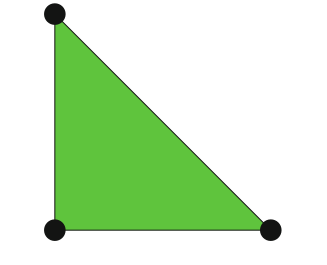
\includegraphics[scale=0.55]{FIgura_16.png}
\caption{ Triángulo de Lagrange con 3 grados de libertad, (Logg et al, 2012)}
\label{Figura16:2}
\end{figure}


\begin{figure}[ht!]
\centering
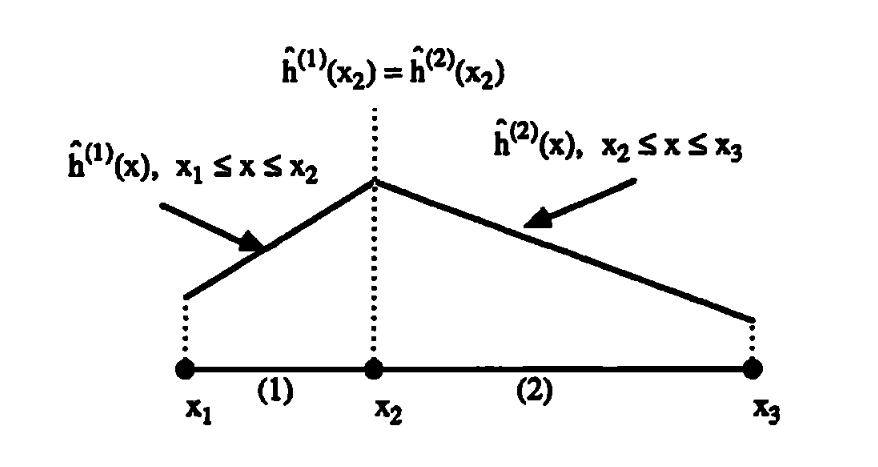
\includegraphics[scale=0.55]{Figura_17.png}
\caption{ Continuidad de la función de interpolación (Istok, 1989)}
\label{Figura17:2}
\end{figure}

Entonces, para garantizar la existencia de la solución $u(x,y,z)$ es necesario que la función de interpolación sea derivable $p$ veces, donde $p$ es el orden de la derivada (y también de la ecuación diferencial). En ocasiones podemos usar técnicas como la integración por partes, para relajar las condiciones de derivabilidad y tener una mayor disponibilidad de funciones base.
\\
\\
La convergencia es otra de las propiedades que deben de cumplir las funciones base para garantizar la existencia de $u$, esto se basa en el hecho de que la función base aproxima la solución $u$ en cada nodo, por lo que usando una función base adecuada, un mayor número de elementos finitos dentro del dominio (mayor número de grados de libertad y menor tamaño de elemento) se aproximara mejor a la solución real $u$, o en otras palabras, la solución converge a la solución real cuando el número de elementos y grados de libertad aumenta. Para encontrar las funciones base que cumplen esta propiedad de convergencia, supongamos que la ecuación \ref{eqn:fe6} que determina la solución $u$, tiene un valor constante $u_{0}$ durante todo el dominio, en términos de flujo, la carga hidráulica es constante dentro de ese elemento, por lo que la ecuación \ref{eqn:fe6} queda de la siguiente forma:

\begin{equation}
\label{eqn:fe19}
\\   u_{0}=\hat{u}^{e}=\displaystyle\sum_{i=1}^n {v_{i}}^{e}(x,y,z)u_{0}
\end{equation}

Despejando la ecuación \ref{eqn:fe19} podemos obtener la regla que modela la carga hidráulica cuando es constante en todo un dominio, y también garantizar la convergencia de la solución para una función base $v$.

\begin{equation}
\label{eqn:fe20}
    \displaystyle\sum_{i=1}^n  v_{i}^{e}(x,y,z) = 1        
\end{equation}

Con lo anteriormente descrito, sabemos las características que deben de tener los componentes de un elemento finito al momento de resolver un problema variacional, y es a partir de las combinaciones de diferentes características de los componentes de la tripleta (\textit{V},\textit{T},\textit{L}), que podemos clasificar nuestros elementos finitos. La primer clasificación se realiza sobre la relación entre la forma de la malla \textit{T} y las funciones base.
\\

Para tener una mayor comprensión sobre las formas que puede adquirir una malla, podemos definir la geometria de cada elemento como una combinación lineal de una función de interpolación con las coordenadas en cada grado de libertad (nodos), de igual forma como definimos la solución $u$ (ecuación \ref{eqn:fe6}), obteniendo una ecuación del siguiente estilo:

\begin{equation}
\label{eqn:fe21}
    \\x(P)=\displaystyle\sum_{i=1}^n  S_{i}^{e}(x,y,z)x_{i}        
\end{equation}

Donde P es un punto cualquiera dentro del elemento y $S_{i}$ es una función de interpolación, que en este caso es llamado función forma y determina la malla \textit{T} de la misma forma que las funciones de interpolación \textit{V} a la solución. De igual forma que con las funciones base, las funciones de forma asumen generalmente funciones lineales aunque pueden también ser de orden cuadráticos o más. El orden de las funciones de interpolación y forma, deben de ser elegidos conforme al tipo de problema que se pretende resolver, por ejemplo, un problema cuyo dominio se puede representar por lineas rectas pero su solución corresponde a valores que asumen por elemento una forma cuadrática; esta combinación de ordenes entre las funciones base y de forma, dan como resultado una clasificación de elementos finitos en tres grupos.
\\

El primer grupo son los \textbf{elementos subparamétricos}, y consisten en el uso de funciones base de mayor orden que sus funciones de forma; en los \textbf{elementos isoparamétricos} el orden de las funciones base y de forma son las mismas; y los \textbf{elementos superparamétricos}, las funciones de forma tienen un mayor orden que las funciones base. Un aspecto importante de esta clasificación es que si ocupamos elementos subparamétricos y superparamétricos, no todos los grados podrán ser evaluados, por lo que es necesario definir bien el tipo de elemento que queremos ocupar. Para efectos de esta tesis, ocuparemos principalmente funciones isoparamétricas y subparamétricas para resolver las simulaciones de flujo de agua subterránea.
\\
\begin{figure}[ht!]
\centering
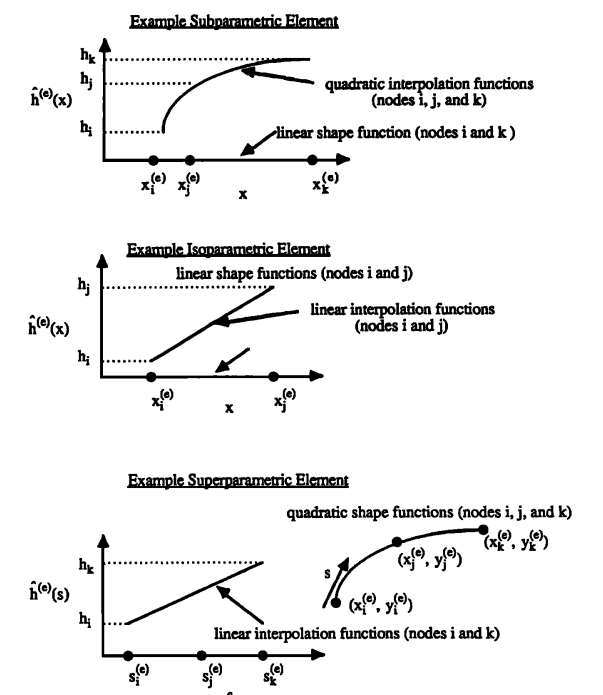
\includegraphics[scale=0.8]{Figura_18.png}
\caption{ Arriba; elemento subparamétrico; Intermedio, elemento isoparamétrico; Abajo, elemento superparamétrico (Istok, 1989).}
\label{Figura18:2}
\end{figure}

Habiendo tratado la geometria de la malla \textit{T} y las funciones base \textit{V}, los grados de libertad \textit{L} se representan de forma esquematizada para cada familia de elementos finitos. Los grados de libertad de cada familia nos permiten hacer una evaluación correcta y una aproximación más cercana al resultado real de la función $u$, además, no solo podemos determinar  los grados de libertad como un punto dentro de una malla, sino que podemos ampliarlo hasta un punto de evaluación en las derivadas, segundas derivadas, componentes direccionales y otros conceptos asociados a la geometría del elemento \textit{T} como función.
\\
\\
Para manejar el concepto anterior, podemos tomar encuenta que \textit{L} es un conjunto de valores que representan los grados de libertad $\textit{L}=\{l_{1},l_{2},...,l_{n}\}$, donde $v(x_{i})$ es una función de las coordenadas donde se encuentran los grados de libertad y que garantiza que $v$ es una base del espacio de funciones \textit{V}. Las formas de definir un grado de libertad son las siguientes \cite{Logg2012}.
\\

\textbf{Punto de evaluación.} Es la forma más común de definir los grados de libertad, consiste esencialmente en asignar el grado de libertad en una punto ubicado por su coordenada $\textbf{x}=(x,y,z)$:

\begin{equation}
\label{eqn:fe22}
    \\l(v)=v(x_{i}),  i=1,...,d        
\end{equation}

donde d es el número de grados de libertad del elemento finito.
\\
\\
\textbf{Evaluación de primeras derivadas.}. Consiste en la evaluación de todas las primeras derivadas de la función $v$ sobre la coordenada de cada grado de libertad:

\begin{equation}
\label{eqn:fe23}
    \\l(v)=  \dfrac{{\partial}v(x_{i})}{\partial{x_{i}}},  i=1,...,d              
\end{equation}

\textbf{Evaluación sobre la componente direccional.}. Es la evaluación sobre un punto definido en \textbf{x} en una dirección \textit{n}:

\begin{equation}
\label{eqn:fe24}
    \\l(v)=  v(x){\cdot}n            
\end{equation}

\textbf{Evaluación sobre la derivada direccional.}. Es la evaluación sobre la derivada de un punto definido en \textbf{x} en una dirección \textit{n}:

\begin{equation}
\label{eqn:fe25}
    \\l(v)=  {\nabla}v(x){\cdot}n            
\end{equation}

Existen otras formas de evaluación de $l(v)$, como en los momentos de $v(x)$ o las derivadas superiores de este, aunque generalmente en la práctica se ocupan sólo la evaluación en un punto y la componente direccional para una formulación mixta.
\\
\\
Las familias de elementos finitos se caracterizan a partir del espacio de funciones en el que se encuentran definidos las funciones base $v$; además, dentro de una misma familia de elementos finitos, existen elementos que no pertenecen al espacio donde se definen sus funciones base $v$, que se conocen como elementos no conformes, mientras que en el caso de pertenecer al mismo espacio de funciones, se denominan elementos conformes.
\\
\\
La familia de elementos más usada en la práctica se encuentran sobre el espacio $H^{1}$ que se ocupa para resolver un problema variacional de una ecuación diferencial cuyo resultado es un campo escalar $u$, este espacio se utiliza principalmente en problemas elípticos de segundo orden como la ecuación de flujo, donde subespacios discretos de $H^{1}$ son ocupados para cada elemento finito. Tipicamente, cada elemento usa espacios de polinomios a partir de funciones suaves por partes sobre las fronteras del dominio, que debe ser continuo sobre el espacio $H^{1}$, un ejemplo conforme de estos espacios, son los tradicionales elementos de Lagrange, mientras que un ejemplo no conforme son los espacios de Crouzeix-Raviart, otros espacios que se pueden usar para discretizar y construir $H^{1}$, son los elementos de Hermite y Arcyris, aunque son poco comunes en la práctica.
\\
\\
Los elementos de Langrage son los más usados para discretizar $H^{1}$, los polinomios que representan la base del espacio se expresan con la notación $P_{i}$, donde i es el grado del polinomio, y la notación general para cualquier elemento de Lagrange es $CG_{q}$, donde q representa la dimensión del elemento. Existe todo una familia de elementos del tipo langrage por cada grado polinomial, que generalizan la interpolación polinómica de Lagrange. Generalmente, se ocupan polinomios de grado 1 para resolver una ecuación diferencial debido a su fácil implementación computacional, sin embargo, polinomios de mayor orden proveen mayor exactitud en el resultado, además, proveen mayor estabilidad en sus propiedades que los elementos lineales.
\\
\\
Un elemento Lagrange ($CG_{q}$) de  dimensión $q$ esta definido por su tripleta de la siguiente manera:

\begin{equation}
\label{eqn:fe26}
    \\T{\in}\{intervalo,triangulo,tetraedro\}
\end{equation}
\begin{equation}
\label{eqn:fe27}
\\V=P_{q}(T)
\end{equation}

\begin{equation}
\label{eqn:fe28}
    \\ l_{i}=V(x_{i}),\quad i=1,...,n(q)
\end{equation}

La dimensión del elemento finito de Lagrange es definido por el grado del polinomio ocupado para definir las funciones base sobre $T$, y el número de grados de libertad $n(q)$ se define de la siguiente forma para cada tipo de geometría:

\begin{equation}
\label{eqn:fe29}
    n(q)= \left\{ \begin{array}{lcc}
             q+1 \qquad  Intervalo  \\
             \\ \dfrac{1}{2}(q+1)(q+2) \qquad Triangulo  \\
             \\ \dfrac{1}{6}(q+1)(q+2)(q+3)  \qquad Tetraedro 
             \end{array}
   \right.
\end{equation}

Mientras que las coordenadas de los puntos $x_{i}$, correspondientes a los grados de libertad, se pueden obtener a partir de la siguiente fórmula:

\begin{equation}
\label{eqn:fe30}
     x= \left\{ \begin{array}{lcc}
             \dfrac{i}{q} \qquad 0{\le}i{\le}q \qquad Intervalo  \\
             \\ (\dfrac{i}{q},\dfrac{j}{q})  \qquad 0{\le}i+j{\le}q \qquad Triangulo  \\
             \\ (\dfrac{i}{q},\dfrac{j}{q},\dfrac{k}{q})  \qquad 0{\le}i+j+k{\le}q \qquad Tetraedro 
             \end{array}
   \right.
\end{equation}

Esta forma de asociar los puntos $x_{i}$, no es única, y se puede tomar en consideración otras formas de acotar los grados de libertad. En general, solo es necesario que los puntos que se encuentren en la frontera puedan ser acoplados con las funciones polinómicas. La \ref{Figura19:2} muestra elementos de diferentes dimensiones, con sus respectivos grados de libertad.
\\

Otra familia de elementos finitos muy usados en la práctica, corresponde a los usados para discretizar el espacio de funciones $L^{2}$ referidos a elementos finitos donde sus elementos no se encuentran en $C^{0}$. Este tipo de elementos son utiles al momento de una formulación mixta donde se pretende encontrar la solución de las cargas hidráulicas a partir del acoplamiento del flujo entre las fronteras de los elementos finitos. El elemento finito más utilizado para discretizar este espacio son los elementos discontinuos de Galerkin (DG), donde el flujo númerico entre las fronteras de los elementos son ensamblados en su formulación integral. Los métodos de Galerkin Discontinuos fueron originalmente desarrollados para EDP's hiperbolicos aunque también son muy útiles en EDP's elipticas y parabolicas.

\begin{figure}[ht!]
\centering
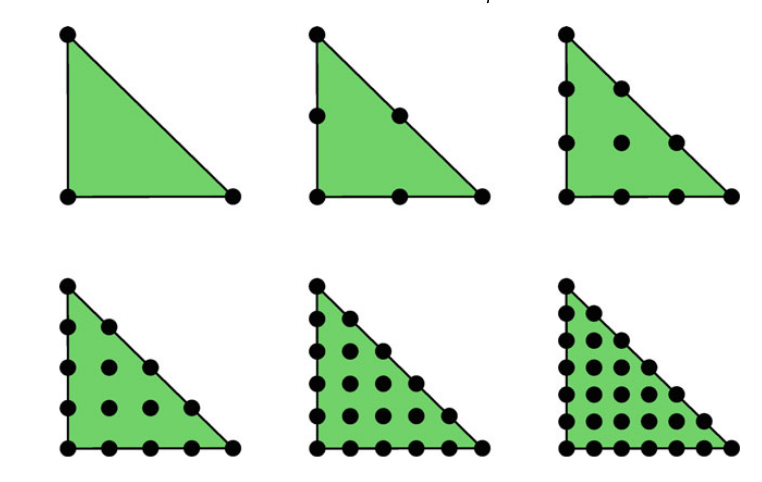
\includegraphics[scale=0.42]{Figura_19.png}
\caption{ Elemento finito triángular para dimensiones q=1,2,3,4,5,6 (Logg et al, 2012) . }
\label{Figura18:2}
\end{figure}

Los elementos de Lagrange Discontinuos ($DG_{q}$) estan definidas por el grado de los polinomios q=0,1,2,..., donde la dimensión del elemento se ve definido por la ecuación \ref{eqn:fe29} y la posición de los grados libertad por la ecuación \ref{eqn:fe30}. La diferencia clave de estos elementos con Langrange Continuo, es que no existe continuidad global, sino que el ensamble se hace elemento a elemento desde el problema variacional.

\begin{figure}[htbp]
\centering
\subfigure[CG]{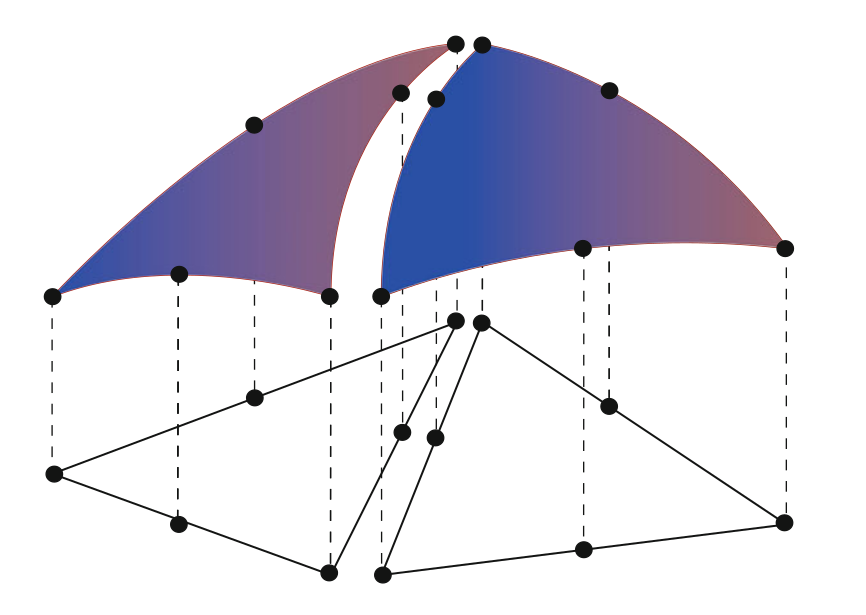
\includegraphics[width=70mm]{Figura_20A.png}}
\subfigure[DG]{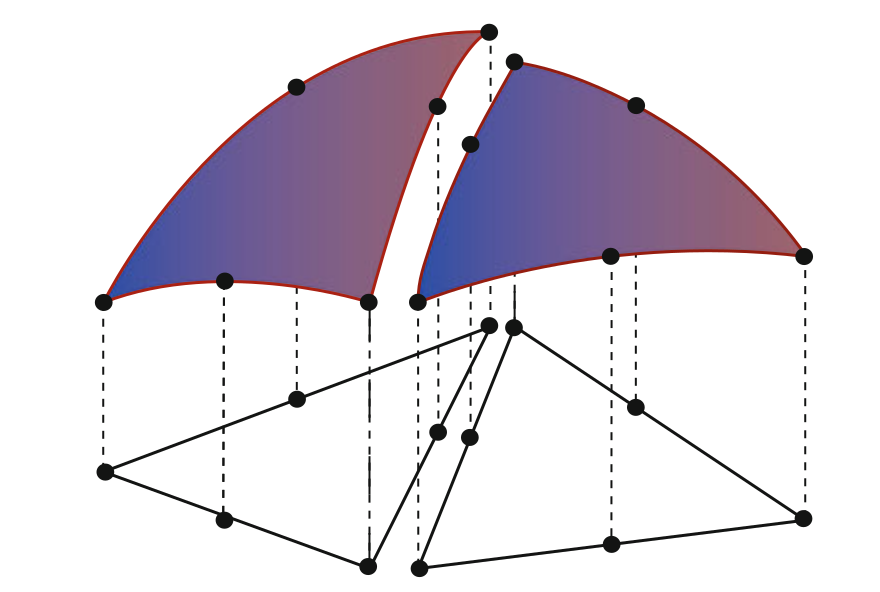
\includegraphics[width=70mm]{Figura_20B.png}}
\caption{Diferencias entre Galerkin Continuo (Derecha) y Discontinuo (Izquierda) (Logg et al, 2012).} \label{Figura19:2}
\end{figure} 


\subsection{Resolución del problema variacional}

Para obtener el campo escalar asociado a la ecuación diferencial parcial, debemos pasar de un planteamiento complejo y abstracto como resulta la ecuación \ref{eqn:fe18} a un problema discreto definido por el tipo de elemento finito que queremos ocupar para resolver el problema. Partiendo de la formulación integral propuesta en la ecuación \ref{eqn:fe18a} y la discretización en un elemento finito de Lagrange (\ref{eqn:fe26}). 
La discretización para obtener la solución $u(x,y,z)$, consiste en definir la función base $v(x)$ a partir de la combinación lineal de funciones interpoladoras $\phi(x)$, que resulta ser una base vectorial para el espacio $H$ y que se extiende sobre los grados de libertad del elemento finito $l(j)$ de la siguiente forma:


 \begin{equation}
 \label{eqn:fe31}
\displaystyle\sum_{j=1}^n  l_{j}(v)\phi_{j}  \quad  j=1,2,..,n(q)     
\end{equation} 

El espacio de funciones que discretiza el espacio \eqref{eqn:fe9} se ve definida por los grados de libertad y la geometría del elemento. 

\begin{equation}
\label{eqn:fe31}
\hat{H}^{1}=  \left[ u(x,y,z) : \quad \displaystyle\sum_{j=1}^n  u_{j}\phi_{j}(x,y,z)  \quad  j=1,2,..,n(q)\right]     
\end{equation}
 
Habiendo definido la discretización de nuestro problema en un elemento finito del dominio, la obtención de nuestra solución en los nodos de evaluación se obtiene al sustituir los elementos del espacio $S^{H}$ en nuestra formulación integral \ref{eqn:fe18a}.

\begin{equation}
 \label{eqn:fe32}
\displaystyle\int_{\Omega}^{} {\nabla}u(x,y,z){\nabla}\phi_{i}(x,y,z)d\Omega   = \displaystyle\int_{\Omega}^{} F(x,y,z)\phi_{i}(x,y,z)d\Omega  - \left. \nabla{u(x,y,z)}\phi_{i}(x,y,z)\right]_{\partial{\Omega}}    
\end{equation}

Donde la función solución $u(x,y,z)$ se incluye como elemento del espacio de funciones $S^{H}$ al igual que su derivada ${\nabla}u(x,y,z)$ de la siguiente forma:

\begin{equation}
\label{eqn:fe33}
\displaystyle\sum_{j=1}^{n(q)}  u_{j}{\nabla}\phi_{j}(x,y,z)  \quad  j=1,2,..,n(q)     
     \end{equation}

En la ecuación \ref{eqn:fe33}, $u_{j}$ es el valor desconocido de $u(x,y,z)$, definida en la malla por el grado de libertad $l(x_{j})$ del elemento finito. Sustituyendo la ecuación \ref{eqn:fe33} en la ecuación \ref{eqn:fe32}, obtenemos la siguiente expresión:

\begin{equation}
 \label{eqn:fe34}
\displaystyle\sum_{j=1}^{n(q)} u_{j} \displaystyle\int_{\Omega}^{} {\nabla}\phi_{j}(x,y,z){\nabla}\phi_{i}(x,y,z)d\Omega   = \displaystyle\int_{\Omega}^{} F(x,y,z)\phi_{i}(x,y,z)d\Omega  - \left. \nabla{u(x,y,z)}\phi_{i}(x,y,z)\right]_{\partial{\Omega}}    
\end{equation}

La ecuación anterior es el problema variacional discretizado en un elemento finito del dominio, donde su desarrollo nos lleva a la resolución de un sistema de ecuaciones lineales que se puede representar en forma matricial:

\begin{equation}
 \label{eqn:fe34}
A\textbf{U}=\textbf{b}
\end{equation} 

Donde la matriz de coeficientes $A$ (también llamada matriz de rigidez), es el resultado del lado izquierdo de la ecuación \ref{eqn:fe33}; $\textbf{U}$ es el vector de incognitas y $\textbf{b}$ es el vector de términos independiente que caracteriza a la fuente del fenómeno físico y las condiciones de frontera.
\\
\\
En cualquier problema que se trate con ecuaciones diferenciales, es necesario definir las condiciones de frontera para garantizar la unicidad de la solución, por lo general, se manejan dos tipos de condiciones de frontera que se implementan de diferente forma dependiendo de la formulación del problema variacional. Las condiciones de Dirichlet (ecuación \ref{eqn:fe35}) tienen la caracteristica de tener un valor constante en las fronteras del dominio del problema, mientras que las condiciones de Neumann (ecuación \ref{eqn:fe36}) definen la frontera a partir del cambio de la función $u$ sobre su frontera.

\begin{equation}
 \label{eqn:fe35}
 u(x_{0},y_{0},z_{0})=f(x,y,z)
\end{equation} 

\begin{equation}
 \label{eqn:fe36}
 {\nabla}u(x_{0},y_{0},z_{0})=g(x,y,z)
\end{equation} 

En la formulación integral de la EDP (ecuación \ref{eqn:fe18a}), podemos observar que aparte del término fuente, al momento de relajar las condiciones de derivabilidad obtenemos una expresión que corresponde a las condiciones de frontera y se ve reflejado en el vector $\textbf{b}$, esta implementación se le conoce como \textbf{condición natural} y dependiendo de la forma en la que se haga la formulación se puede tratar de una condición de Dirichlet o Neumann, en caso que la condición de frontera no se defina dentro del problema variacional, se define dentro del espacio de funciones $S^{h}$ como un subconjunto del mismo, donde la frontera se define por la función $f(x,y,z)$ y se le conoce como \textbf{condiciones esenciales}.
\\
\\
La solución del sistema definido en la ecuación \ref{eqn:fe36}, es también llamada solución local debido a que se resuelve sobre un elemento del dominio $\Omega$. La solución global consiste en el ensamblaje de todos los elementos que conforman al dominio para conseguir una matriz de rigidez global de dimensiones $nxn$, donde $n$ seria el número de incognitas a resolver. El ensamblaje de los elementos finitos es posible a partir de la definición de coordenadas locales y globales que garanticen la continuidad de la solución en la frontera con cada elemento, donde finalmente se obtiene la solución de problema a partir de algún método númerico para sistemas de ecuaciones lineales, como Gauss-Seidel o SOR. 
\\
\\

\begin{figure}[ht!]
\centering
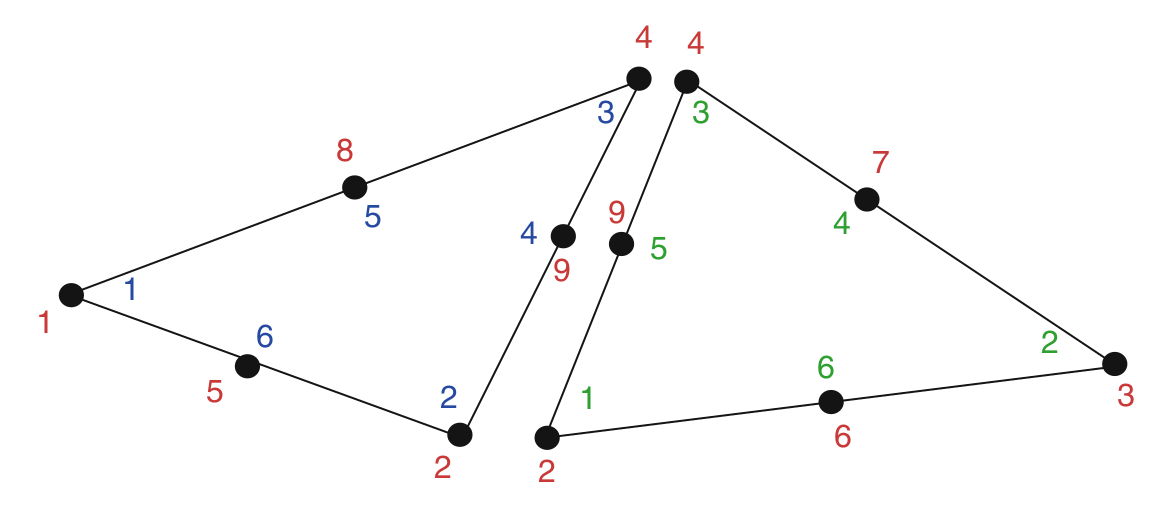
\includegraphics[scale=0.55]{Figura_21.png}
\caption{ Ensamblaje de elementos finitos (Logg et al, 2012)}
\label{Figura20:2}
\end{figure}

En términos generales, los pasos necesarios para resolver una ecuación diferencial parcial a partir del método de elementos finitos, son los siguientes:

\begin{enumerate}
\item  Dada la EDP que modela el fenómeno físico, discretizar el dominio $\Omega$ en una malla que puede ser definida por las funciones forma.
\item  Deducir la formulación integral de la EDP a partir del método de residuos ponderados o el método variacional.
\item Considerando la discretización del dominio, elegir el espacio de funciones para construir la solución del problema variacional. Definiendo la tripleta que caracteriza el tipo de elemento finito.
\item Definir el sistema de ecuaciones lineales a partir de la discretización del problema y el espacio de funciones elegido. Resolver las derivadas e integrales de las funciones de interpolación (función peso) y el sistema de ecuaciones a partir de método númericos \cite{Logg2012} \cite{Istok1989} \cite{Whiteley2017}.
\end{enumerate}


\section{Implementación computacional}   

La ecuación de flujo estacionaria es una ecuación diferencial parcial elíptica, cuyo campo de cargas hidráulicas y de flujo serán tratados como objetos en $Python$ y obtenidos a partir de DOLFIN, la interfaz gráfica de FeniCS. 

\subsection{Implementación con FeniCS}

La resolución de una EDP con FeniCS requiere de tres objetos principales: la formulación integral(con el espacio discreto implementado), las condiciones de frontera esenciales y el campo de cargas hidráulicas donde se obtendran los resultados.
\\
\\
El elemento finito queda definido por su tripleta, la cuál consiste en la discretización del dominio $\Omega$ con las celdas $T$, en FeniCS crearemos la malla con la forma de los elementos como un objeto de tipo $\textit{Mesh}$, donde definimos las dimensiones de nuestra malla, asi como la refinación de la misma. Para las simulaciones realizadas, haremos la resolución del problema en dos mallas, una de $[20{\times}10]$ elementos triángulares, y otra más refinada de $[40{\times}20]$ elementos.
\\

\begin{figure}[htbp]
\centering
\subfigure[200 elementos finitos]{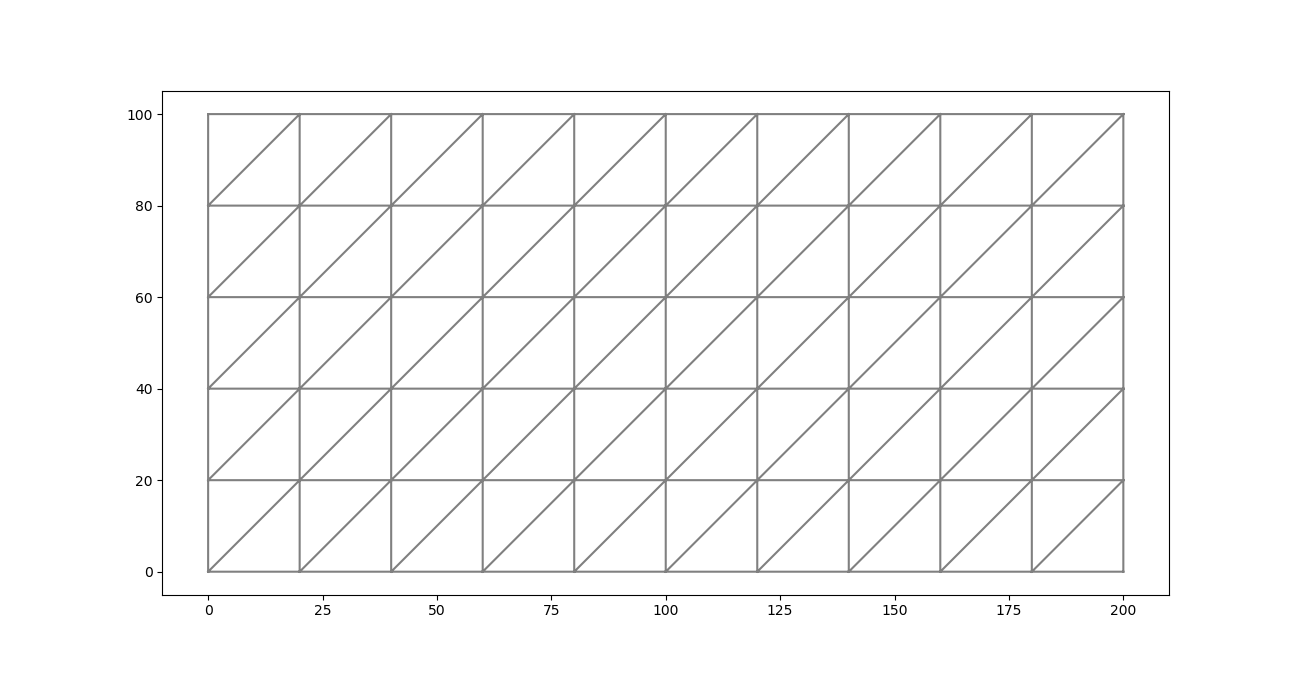
\includegraphics[width=70mm]{Figura_24A.png}}
\subfigure[400 elementos finitos]{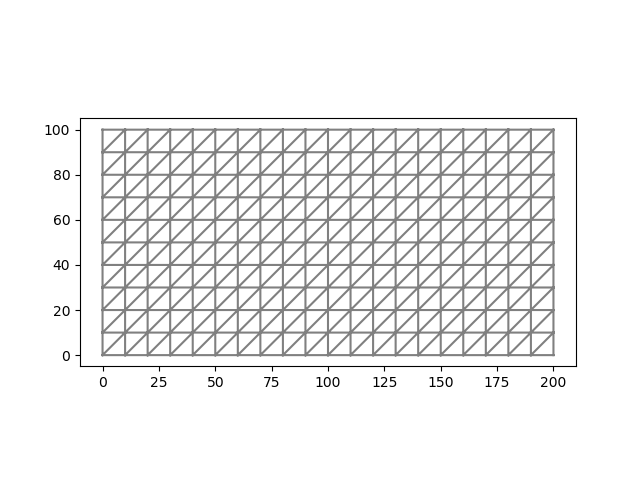
\includegraphics[width=60mm]{Figura_24B.png}}
\caption{Diferente refinación mallas}
 \label{Figura19:2}
\end{figure}

Posteriormente, se define el espacio de funciones que se ocupara para obtener el campo de cargas hidráulicas, como se vio en la sección anterior, el más usado para este tipo de ecuaciones son los elementos de Lagrange, cuyo incremento en el orden de los polinomios de interpolación aumenta la dificultad del cálculo pero incrementa la exactitud de la solución. El elemento finito se crea a partir de la función $\textit{FunctionSpace}$ cuyos argumentos de entrada son el objeto malla (que incluye los grados de libertad), el tipo de funciones de interpolación y el grado de las funciones.

\lstset{language=python,breaklines=true,belowskip=1.3em, aboveskip=2em\footnotesize}
\begin{lstlisting}[frame=single]
mesh= RectangleMesh(Point(0,0),Point(200,100),10,5)
EF = FunctionSpace(mesh, 'P', 1)
\end{lstlisting}
    
Las fronteras esenciales para el caso de una formulación tradicional son las condiciones de Dirichlet, que se definen a partir 
de la función $\textit{DirichletBC}$, cuyos argumentos de entrada son el elemento finito (espacio de funciones) creado anteriormente, la función que determina los valores en la frontera (ecuación \ref{eqn:fe35}) y una función que indique la posición donde se encuentra la frontera en la malla.

\lstset{language=python,breaklines=true, basicstyle=\footnotesize}
\begin{lstlisting}[frame=single]
Frontera = DirichletBC(EF, f(x), Marcador_Frontera)
\end{lstlisting}

La función f(x) puede ser constante o una expresión en función de las coordenadas de la malla, mientras que el marcador de la frontera se define a partir de una condicional que asigna en la malla el valor de 1 en la zona de frontera y 0 en el resto de los puntos de la malla, un ejemplo de un marcador de frontera en el lado izquierdo de una malla es el siguiente:

\lstset{language=python,breaklines=true, basicstyle=\footnotesize}
\begin{lstlisting}[frame=single]
def frontera_I(x,frontera):
 tol=1E-14 
 if frontera:
  if abs(x[0])<=tol: 
   return True
  else:
   return False 
 else:
  return False
\end{lstlisting}

La definición de las condiciones esenciales es de vital importancia, ya que una mala delimitación podria llevarnos a errores de cálculo. Después de generar las condiciones esenciales para toda la frontera, es necesario obtener la formulación integral de nuestra EDP. FeniCS permite la creación de términos matemáticos abstractos apartir del componente UFL, por lo que solo es necesario definir un objeto en el espacio de funciones de Lagrange como la función solución $u$, y un objeto definido en el mismo espacio $v$ que sirva como función  test (o base) para finalmente definir nuestra formulación integral.

\lstset{language=python,breaklines=true, basicstyle=\footnotesize}
\begin{lstlisting}[frame=single]
u=TrialFunction(V)
v=TestFunction(V)
f=Constant(0)
a=dot(grad(u),grad(v))*dx
g=Constant(0)
L=f*v*dx-g*v*ds
\end{lstlisting}

De esta forma obtenemos la formulación integral con el espacio de funciones discretizado en función del elemento finito. La solución del problema se obtiene de forma automática con la función $\textit{solve}$, donde los argumentos son las condiciones esenciales obtenidas con la función $\textit{DirichletBC}$, la formulación integral, y un campo de cargas hidráulicas inicial de ceros que se obtiene a partir de la malla con el comando $\textit{Function}$.

\lstset{language=python,breaklines=true, basicstyle=\footnotesize}
\begin{lstlisting}[frame=single]
u= Function(V)
solve(a==L,u,Frontera)
\end{lstlisting}

El resultado final de la tesis es obtener no solo la distribución del campo de cargas hidráulicas, sino también la distribución del flujo o descarga especifica del agua por cada elemento finito, dada por la ecuación de darcy (ecuación 1.4). El gradiente de las cargas hidráulicas se obtiene a partir de la aplicación del operador $\textit{grad()}$ al campo $u$, donde conseguimos el valor del flujo al multiplicar el vector gradiente de cargas hidráulicas del centroide en cada elemento por su conductividad hidráulica. La gráfica de los resultados se realizá con la biblioteca $Matplotlib$. 

\subsection{Implementación de la heterogeneidad}

Obtener las cargas hidráulicas de la ecuación de flujo es un proceso simple con FeniCS que se complica dependiendo del grado de complejidad de nuestro problema. La implementación de la heterogeneidad se aborda en esta tesis desde dos enfoques; la heterogeneidad simple, que consiste en un dominio fraccionado en partes con diferentes conductividades hidráulicas, que geologicamente representa un cambio brusco lateral de facies o un cambio de litologia de un estrato a otro, donde la asignación de la conductividad hidráulica será dependiendo del modelo geológico que se trabaje. El otro tipo es la heterogeneidad aleatoria, donde el campo de conductividades hidráulicas en cada elemento finito es representado por una función aleatoria; que geológicaménte representa la variación de conductividad hidráulica en un material a pequeña escala.
\\
\\
La implementación del primer tipo de heterogeneidad se realiza de forma similar que la creación de las condiciones de Dirichlet, creando un marcador del dominio para cada tipo de material para posteriormente asignar a cada punto marcado la conductividad hidráulica que le corresponde, una forma simple de implementar el marcado y la asignación de conductividades es creando una clase de objetos que definan la heterogeneidad a partir de dos funciones; la primer función consiste en la lectura de los valores de conductividad hidráulica como atributos y la segunda en la asignación de la conductividad hidraulica  en una zona determinada por condicionales.


\lstset{language=python,breaklines=true, basicstyle=\footnotesize}
\begin{lstlisting}[frame=single]
class K(Expression):
 def set_k_values(self, k_0, k_1):
     self.k_0, self.k_1 = k_0, k_1
 def eval(self, value, x):
   tol = 1E-14 
   if  tol + 100 <= x[0] <= 150 + tol:
      value[0] = self.k_0
   else:
      value[0] = self.k_1
\end{lstlisting}

Posteriormente se crea un objeto de esta clase y se le asignan como atributos las conductividades hidráulicas. 

\lstset{language=python,breaklines=true, basicstyle=\footnotesize}
\begin{lstlisting}[frame=single]
Conductividad = K(degree=1)
Conductividad.set_k_values(10,1)
\end{lstlisting}

Esta definición de heterogeneidad tiene la dificultad de estar definida por reglas matemáticas simples, por lo que si se requieren formas más complejas dentro del dominio, es necesario primero realizar el marcado del dominio para cada material (puede generarse la malla con herramientas externas y luego importarse) y después hacer la asignación de conductividades. Para obtener los valores de carga hidráulica en medios heterogéneos simples, se realiza la multiplicación del objeto donde estan definidas nuestras conductividades y su distribución por su formulación integral. Finalmente se hace la resolución de forma usual y se sigue el procemiento descrito al final de la sección anterior.
\\
\\
La heterogeneidad aleatoria se fundamenta en la teoría de la geoestadística, donde para obtener el campo de conductividades hidráulicas en cada elemento, buscaremos reproducir la función aleatoria K(\textbf{x}) caracterizado por un semivariograma teórico $\gamma(h)$ en el centroide de cada elemento, este procedimiento es conocido como \textbf{simulación no condicional} \cite{Quintin2000}.
\\
\\
La implementación de la simulación no condicional se realiza a través del lenguaje $\textit{R}$, que se ocupa principalmente para cálculos estadísticos a partir de las bibliotecas de análisis geoestadistico $\textit{Gstat}$. Para calcular el campo de conductividades hidráulicas primero es necesario hacer el cálculo del centroide de cada elemento finito, esta va a depender de la forma en la que se halla definido la geometría del elemento (triangular o rectangular) y del número de elementos finitos en la malla, para efectos de esta tesis, se ocupó un algoritmo de cálculo de centroides para una malla regular de elementos triángulares (Apendice B.2)\cite{Beer2010}. 

\begin{figure}[ht!]
\centering
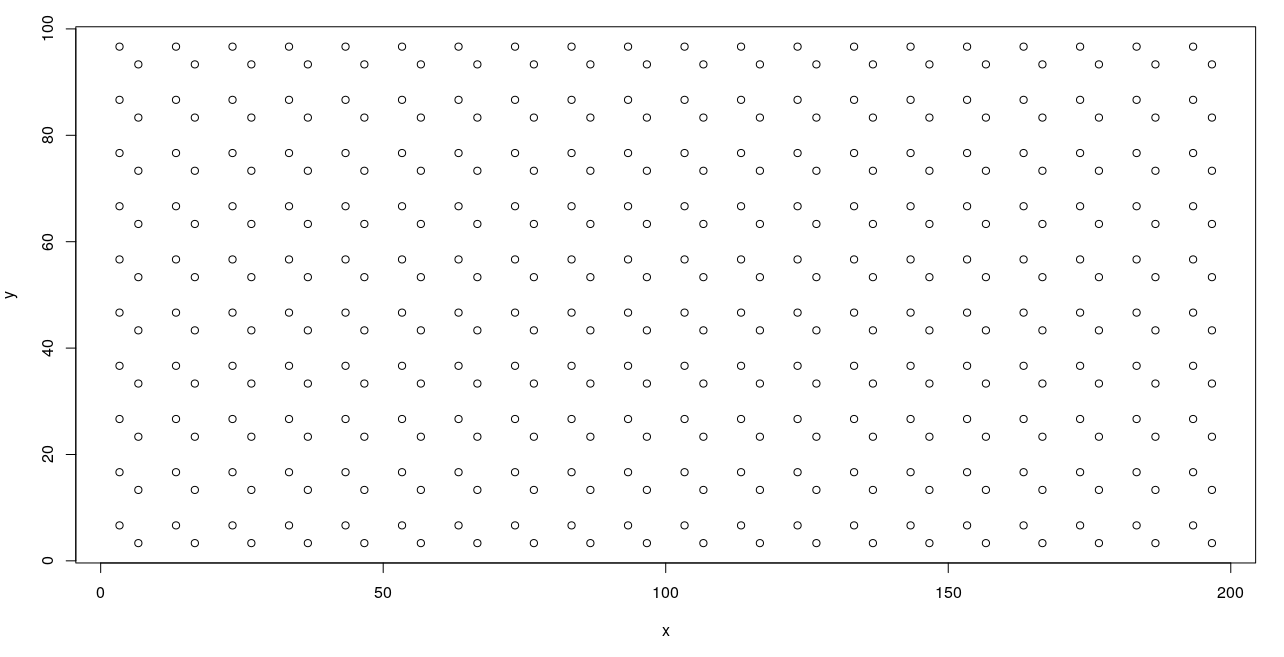
\includegraphics[scale=0.45]{Figura_22.png}
\caption{ Centroides para cada elemento de una malla regular }
\label{Figura20:2}
\end{figure}

Después de obtener la posición de los centroides, se obtiene el semivariograma a utilizar a partir del comando $\textit{vgm}$ que se define a partir de tres valores de entrada, el sill, el tipo de variograma teórico y el rango (veáse sección 1.2.2). A partir del variograma teórico y la posición de los centroides obtendremos el campo de conductividades con los comandos $gstat()$ y $predict()$ \cite{Gonzalez2000} \cite{Pebesma2014}.

\lstset{language=r,breaklines=true, basicstyle=\footnotesize}
\begin{lstlisting}[frame=single]
vgm1=vgm(1,"Exp",15)
g.dummy <- gstat(formula = z~1, locations = ~x+y, dummy = TRUE, beta = 0,model = vgm1, nmax = 20)
yy <- predict(g.dummy, newdata = xy, nsim = 4)
\end{lstlisting}

Como se trato en la sección 1.2.1, las conductividades hidráulicas en una misma formación tienden a tener una distribución log-normal y de la misma forma $gstat$ maneja la aplicación  $X=ln(K)$ a sus datos, por lo que los resultados se presentan con una distribución normal presentandonos valores negativos que no tienen significado físico, por lo que es necesario aplicar la transformación inversa $K=exp(X)$ a los datos obtenidos de la simulación no condicional.
 \\
 \\
Con las conductividades calculadas para cada elemento, la implementación en FeniCS puede hacerse de forma similar que la heterogeneidad simple, aunque es necesario agilizar el proceso de marcado debido a que se tendria que trabajar con un archivo por cada elemento, lo que resulta ineficiente y tardado, para evitar esto, se ocupa un ciclo dentro del código de marcaje, que en conjunto con el comando de FeniCS $\textit{cells(mesh)}$, marca cada elemento finito con un número distintivo.

\begin{figure}[ht!]
\centering
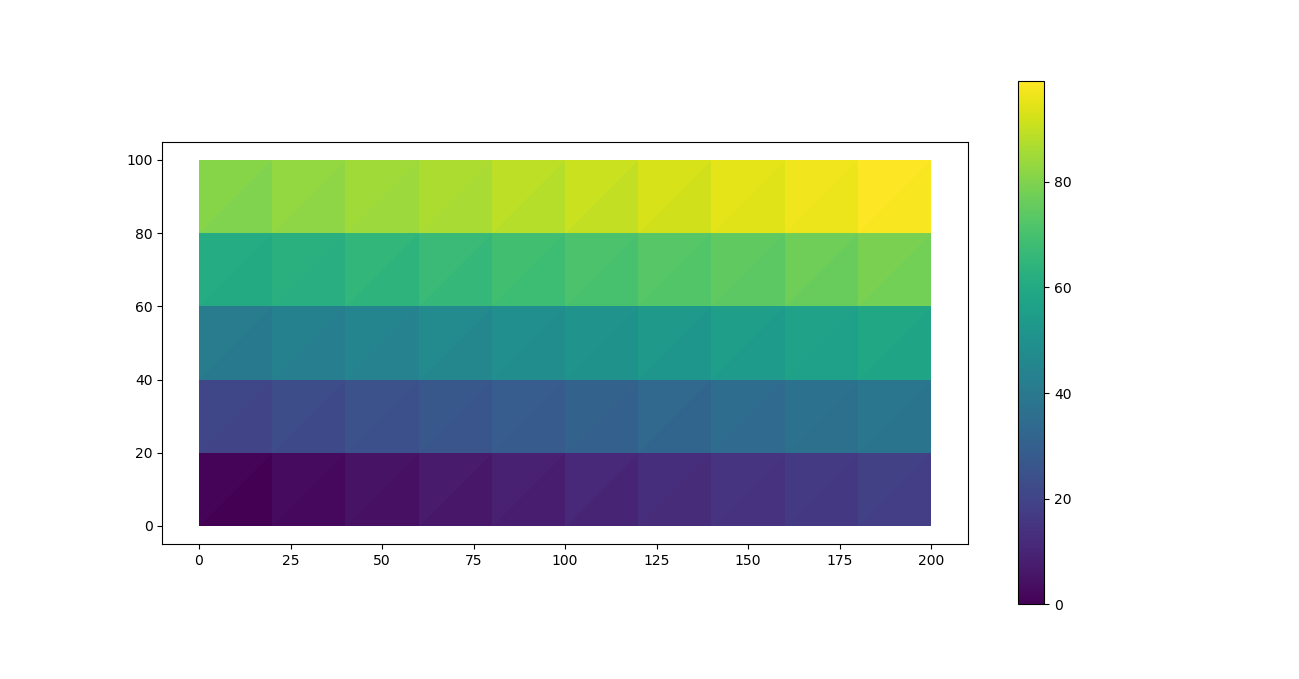
\includegraphics[scale=0.55]{Figura_23.png}
\caption{ Malla marcada por elemento}
\label{Figura20:2}
\end{figure}

Con la malla marcada, el siguiente paso es hacer la asignación para cada elemento con las conductividades obtenidas en $\textit{Gstat}$. Esto se realiza definiendo un objeto $"k"$ como una función en un espacio de funciones del tipo Galerkin Discontinuo, que es el más apropiado para definir la heterogeneidad debido al tratamiento individual que hace sobre cada elemento \cite{Dolejsi2016}, y después, con un ciclo, hacer la asignación de los valores de conductividad hidráulica para cada elemento finito en el objeto "k".

\lstset{language=python,breaklines=true, basicstyle=\footnotesize}
\begin{lstlisting}[frame=single]
# Se realiza el marcado de la malla
k=range(0,400,1)
subdomains=CellFunction('size_t',mesh,0)
cont=0
for cell in cells(mesh):
 subdomains[cell]=k[cont]
 cont=cont+1

plt.figure()
im1=plot(subdomains)
print(subdomains)
plt.colorbar(im1)

# Se crea un espacio de funciones que simbolizan la conductividad hidraulica   
V0= FunctionSpace(mesh,"P",0)
k=Function(V0)

 cont=cont+1
\end{lstlisting}

\lstset{language=python,breaklines=true, basicstyle=\footnotesize}
\begin{lstlisting}[frame=single]

# Se asigna para cada valor del marcado un valor del conjunto de conductividades
ka = np.loadtxt("Pruebayy.txt",delimiter=',',skiprows=1,usecols=[6])
k_values=np.exp(ka)
cont=0
for cell_no in cells(mesh):
 subdomain_no=subdomains[cell_no]
 k.vector()[cont]=k_values[subdomain_no]
 cont=cont+1
\end{lstlisting}



Finalmente, de igual forma que en la  heterogeneidad simple, la conductividad se implementa en la formulación integral y se obtiene la solución con el comando $\textit{solve}$. Para obtener el valor del flujo, se aplica la ecuación de Darcy para el centroide de cada elemento. 



